\documentclass[11pt]{article}

\author{Groep 6:\\
		Niels Desair\\
		Bram Kelchtermans\\
		Dylan Toirkens}
		
\title{\textbf{Studie van meetbare objectieven en ontwerpprincipes van Shneidermann}}

\date{12/10/2016}

\usepackage{graphicx}
\usepackage{parskip}
\usepackage{float}

\begin{document}
	\begin{titlepage}
		
		\newcommand{\HRule}{\rule{\linewidth}{0.5mm}} % Defines a new command for the horizontal lines, change thickness here
		
		\begin{center} % Center everything on the page
			
			\textsc{\LARGE Universiteit Hasselt}\\[1.5cm] % Nme of your university/college
			\textsc{\Large Humane en sociale aspecten van de informatica}\\[0.5cm] % Major heading such as course name
			
			\HRule \\[0.4cm]
			{ \huge \bfseries Studie van meetbare objectieven en ontwerpprincipes van Shneidermann}\\[0.4cm]
			\HRule \\[1.5cm]
			
			\begin{minipage}{0.4\textwidth}
				\begin{flushleft} \large
					\emph{Groep 6:}\\
					Niels \textsc{Desair} \newline
					Bram \textsc{Kelchtermans} \newline
					Dylan \textsc{Toirkens}
				\end{flushleft}
			\end{minipage}
			~
			\begin{minipage}{0.4\textwidth}
				\begin{flushright} \large
					\emph{Datum:}\\
					12 Oktober 2016
					\emph{Academiejaar: } \\
					2016-2017
				\end{flushright}
			\end{minipage}\\[4cm]
			\vspace{40 mm}
			
\includegraphics[width=3.0cm]{UHasselt-logo.jpg}\\[2.0cm]  
		\end{center}
	\end{titlepage}

\section{Inleiding}
In deze studie willen wij kijken of een computerprogramma dat dagelijks door duizenden mensen gebruikt wordt goed scoort bij de meetbare objectieven en de principes van Shneidermann. Het programma dat we hiervoor gekozen hebben, is Google Chrome. Deze browser is al enkele jaren de populairste en geniet van een zeer groot aantal gebruikers en wij denken dat de User Interface daar wel iets mee te maken zou kunnen hebben.
\newpage

\section{Bespreking Niels}
individuele bespreking meetbare objectieven en principes van Shneiderman door student 1 (twee tot drie bladzijden, 800 à 1200 woorden)
\subsection{Meetbare objectieven}
\subsection{Ontwerpprincipes van Shneidermann}
\newpage

\section{Bespreking Bram}
In dit deel bespreekt Bram Kelchtermans zijn bevindingen over de gekozen software. Als meetbare human-factor objectieven heeft hij gekozen voor "Subjective satisfaction", "Speed of Performance" en "Error Rate". Verder wordt er ook nog gesproken over de "Ontwerpprincipes van Schneidderman" toegepast op de gekozen software.
\subsection{Meetbare objectieven}
\subsubsection{Subjective Satisfaction}
Voor de meetbare human-factors objectieven heb ik "subjective satisfaction" gekozen als het belangrijkste aspect. Dit omdat er veel concurrentie is op het vlak van web browsers, hierbij zijn zo goed als alle web browsers gratis. Daardoor is het dus belangrijk dat de gebruikers tevreden zijn over het ontwerp en de werking van Chrome als Google wil dat Chrome consistent gebruikt blijft worden. De gebruiker kan namelijk gemakkelijk en gratis overstappen naar een alternatief zoals bijvoorbeeld Mozilla Firefox. Het lijkt me dus duidelijk dat dit een zeer belangrijk objectief is om na te streven door de ontwerpers. Persoonlijk vind ik dat Google hier zeker op vooruit is gegaan. Dit doordat ze de mogelijkheid geven aan de gebruikers om Chrome aan te passen naar zijn of haar voorkeuren. Denk zo maar aan de ad-block software die er voor zorgt dat alle reclame op sites verdwijnt. Dit is voor vele gebruikers een rede om Chrome te gebruiken. 
\subsubsection{Speed of Performance}
Een ander belangrijk aspect vind ik persoonlijk de "speed of performance". Als we de verschillende gebruikers bekijken bekomen we dat we zowel particulieren als commerciële gebruikers hebben.Het is dus zeer belangrijk voor beide groepen dat het programma dus een snelle verbinding tot het wereldwijde web voorziet. Zoals hierboven al besproken is, kan de gebruiker makkelijk overstappen naar de concurrent als deze sneller is. Op dit vlak is Chrome nog steeds één van de pioniers. Een nadeel is echter dat de eventueel geïnstalleerde plugins en extensions er voor kunnen zorgen dat het surfen minder vlot verloopt. Een goed voorbeeld van dit probleem is de Hangouts extensie. Wanneer deze geïnstalleerd is, werkt Chrome aanzienlijk trager waardoor de gebruiker geneigd zal zijn deze extensie te verwijderen.
\subsubsection{Error Rate}
Tenslotte zou ik het nog willen hebben over de "error rate" van Chrome. Het is belangrijk dat er zo weinig mogelijk fouten optreden bij het gebruik van een webbrowser. Wanneer het programma bijvoorbeeld crashed bij een bepaalde actie zal de gebruiker zich snel genoodzaakt voelen om een alternatief te vinden. Uit persoonlijke ervaring kan ik zeggen dat er meer fouten optreden bij het gebruik van Chrome als vroeger. Persoonlijk denk ik dat dit komt door een te groot aanbod aan extensies en plugins. Dit kan er voor zorgen dat bij het openen van bepaalde sites het programma crashed doordat een plugin niet goed werkt of vast loopt.
\subsection{Ontwerpprincipes van Shneidermann}
\subsubsection{Herken de diversiteit}
Er zijn veel gebruikersgroepen als we het hebben over web browsers. Zowel particulieren als bedrijven maken vaak gebruik van web browsers. In deze twee groepen kunnen we dan weer onderscheid maken in beginnende gebruikers, gebruikers met gemiddelde kennis en expert gebruikers. 
\linebreak
Beginnende gebruikers zullen eerst moeten leren hoe een web browser werkt. Dit heeft echt weinig tot geen gevolgen voor de gebruiksfactor van Chrome. Dit doordat elke web browser via hetzelfde principe werkt en dus altijd aangeleerd zal moeten worden. Er wordt dus geen risico gelopen dat beginnende gebruikers zullen overstappen naar de concurrent. Voor beginnende gebruikers voorzien ze wel de nodige feedback, dit speelt zeker in het voordeel van Chrome. Denk maar aan de hulp die chrome biedt wanneer de gebruiker internetproblemen heeft, zoals te zien is in Figuur \ref{fig:nocon}.
\begin{figure}
  \centering
    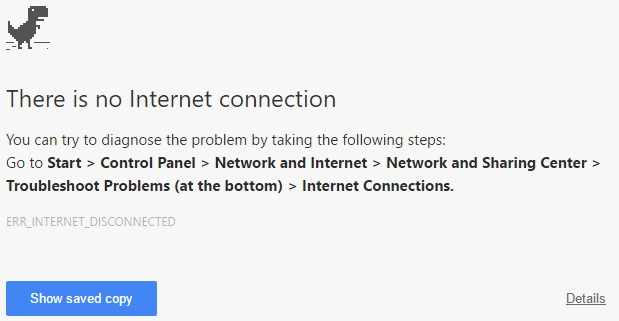
\includegraphics[width=0.7\textwidth]{NoConnection.jpg}
  \caption{Gebruiker heeft geen internetverbinding}
  \label{fig:nocon}
\end{figure}
Deze melding geeft in stappen weer wat de gebruiker moet doen om het probleem op te lossen. Beginnende gebruikers kunnen deze informatie zeker gebruiken en dit speelt dan ook in het voordeel van Chrome.
\newpage
Gebruikers die al wat ervaring hebben met surfen op het web zullen ook sneller de voorkeur geven aan Chrome. Dit doordat Chrome zeer simplistisch is als we over de lay out spreken. Voor de verdere functionaliteitne moet de gebruiker in de menu's navigeren, ook zijn er speciaal voorziene pagina's (zoals de pagina die te zien is in Figuur \ref{fig:apps}). De gebruiker die meer uit zijn of haar browser wil halen kan op deze pagina terecht om de functionaliteiten uit te bereiden. Zo komen we bij de gebruikers die al veel ervaring hebben met Chrome
\newline
Gebruikers die Chrome al lange tijd gebruiken zullen meer functionaliteiten ter beschikking kunnen krijgen als zij dat willen. Denk zo maar aan GMail, Google Drive... al deze applicaties zijn geoptimaliseerd voor Chrome. Een ander groot voordeel dat de gebruikers zullen ondervinden is het feit dat Chrome ge mogelijkheid biedt om de gegevens te synchroniseren tussen de verschillende apparaten. Denk zo maar aan de surf geschiedenis die ook te vinden zal zijn op de mobiele telefoon van de gebruiker. Dit speelt zeker in het voordeel van Chrome. Gebruikers krijgen ook de mogelijkheid om plugins te installeren om het surfen aangenamer te maken, dit is echter niet essentieel. Beginnende gebruikers kunnen profiteren van de snelheid die Chrome biedt, terwijl Chrome voor expert gebruikers de mogelijkheid biedt om de browser aan te passen aan de verschillende eisen van de gebruikers.
\begin{figure}
  \centering
    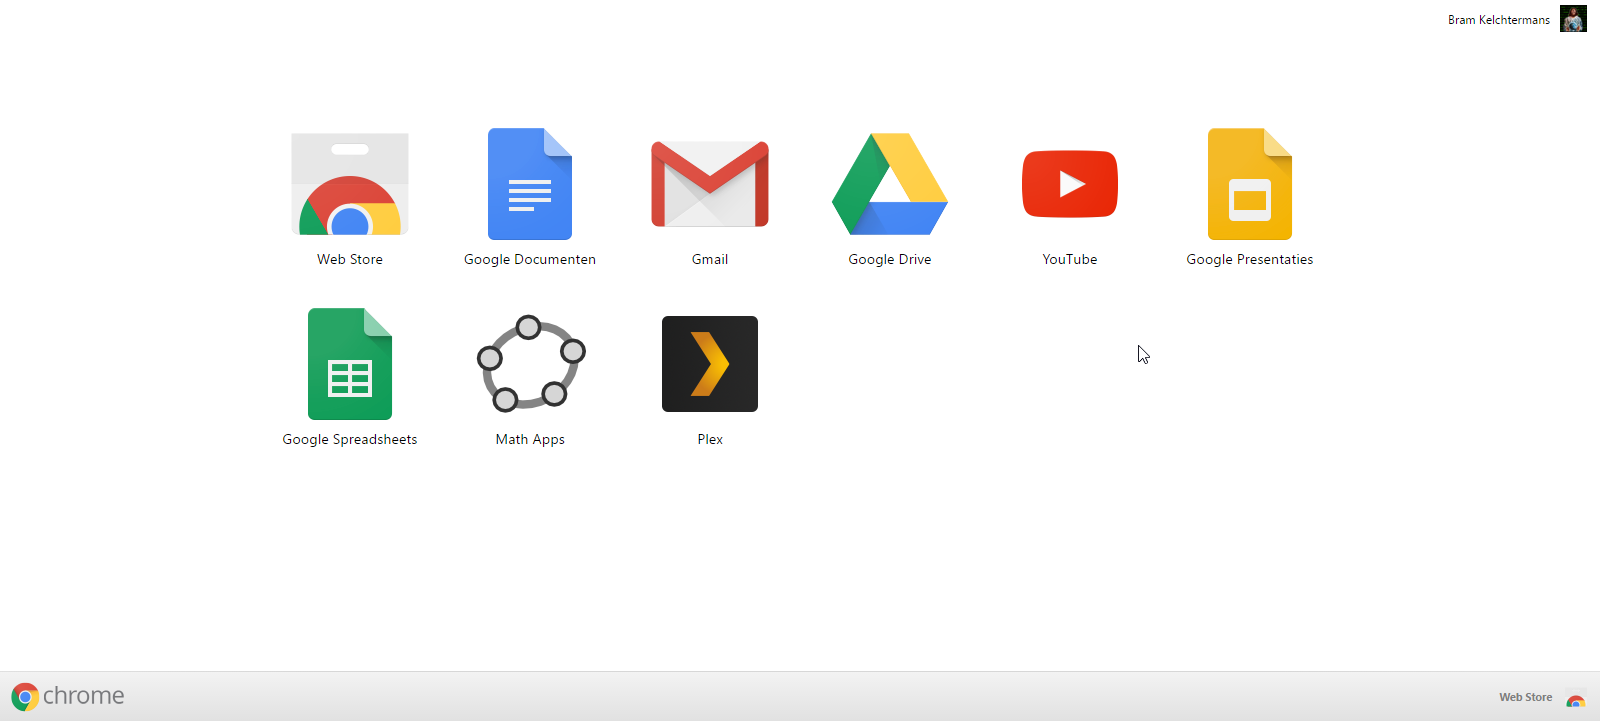
\includegraphics[width=0.9\textwidth]{apps.png}
  \caption{Applicatie pagina van Chrome}
  \label{fig:apps}
\end{figure}
\newpage
\subsubsection{De acht gouden regels voor interface design}
\begin{itemize}
\item Streven naar Consistentie
\newline
Bij browsers is het belangrijk dat er consistent gebruik wordt gemaakt van zowel de lay out als de gebruikte icoontjes. Dit is zeker het geval, zoals te zien is in Figuur \ref{fig:tabsChrome}. Zoals in elke web browser wordt er gebruik gemaakt van dezelfde lay-out om verschillende tabbladen aan te geven of de adresbalk te tonen. Dit is belangrijk doordat de gebruiker hierdoor het programma sneller leert te gebruiken.
\begin{figure}
  \centering
    
\includegraphics[width=0.9\textwidth]{Tabs_Chrome.png}
  \caption{Het lint van Chrome}
  \label{fig:tabsChrome}
\end{figure}
\item Frequente gebruikers toelaten schortcuts te gebruiken
\newline
De gebruikers kunnen hun favoriete pagina's opslaan als bladwijzers. Deze zijn terug te vinden onder de adresbalk (zie Figuur \ref{fig:tabsChrome}). Dit zorgt er voor dat belangrijke pagina's snel toegankelijk zijn, hierdoor wordt de efficiëntie verhoogd.
\item Informatieve feedback aanbieden
\newline
Een voorbeeld hier van is te zien in afbeelding \ref{fig:nochanges}. De gebruiker probeert hier de pagina te verversen terwijl er een wijziging is aangebracht op de pagina die niet bevestigd is. In dit geval wil de gebruiker een post plaatsen op Facebook maar heeft deze nog niet ingediend. Chrome geeft hier een melding van zodat de gebruiker geen data verliest.
\begin{figure}
  \centering
    
\includegraphics[width=0.9\textwidth]{No_Changes.png}
  \caption{Feedback in Chrome}
  \label{fig:nochanges}
\end{figure}
\newpage
\item Dialogen ontwerpen zodat onverwachte resultaten uitgesloten worden en de voortgang duidelijk is.
\newline
In het vorige puntje wordt er al een dergelijk dialoog besproken.
Een ander voorbeeld van dit puntje is te vinden in Figuur \ref{fig:privatecon}. De gebruiker krijgt hier een melding dat de site niet veilig is voor de privacy van de gebruiker. De gebruiker krijgt echter wel nog de mogelijkheid om verder te surfen naar de gekozen website door op "Advanced" te klikken. Zo weet de gebruiker dat Chrome niet garandeerd dat zijn of haar privacy veilig is.
\newline
\begin{figure}
  \centering
    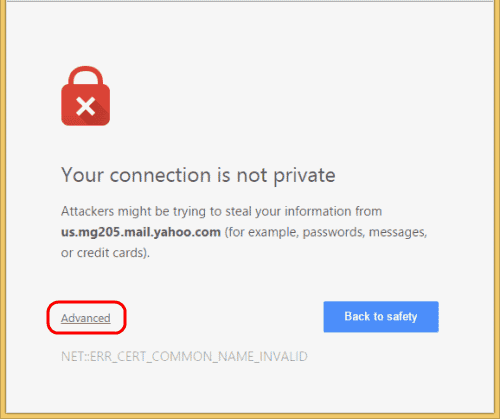
\includegraphics[width=0.9\textwidth]{Chrome-Advanced.png}
  \caption{Onveilige pagina in Chrome}
  \label{fig:privatecon}
\end{figure}
Een ander voorbeeld is te zien in Figuur \ref{fig:loading}, hier kan de gebruiker zien dat de gevraagde pagina geladen wordt. Dit doordat naast de naam van de pagina een laad icoontje te zien is. Hierdoor weet de gebruiker dat hij of zij nog even moet wachten om het gewenste resultaat te bekomen.
\begin{figure}
  \centering
    
\includegraphics[width=0.4\textwidth]{Loading.png}
  \caption{Pagina laden in Chrome}
  \label{fig:loading}
\end{figure}
\item Foutpreventie 
\newline
Een voorbeeldje hier van is niet makkelijk te vinden. Het is logisch dat een web browser zo vlot mogelijk moet werken en dus weinig fouten mag genereren. Wat bij Chrome een voordeel is, is de integratie van de zoekmachine in de adresbalk. Dit kan gezien worden als foutpreventie. In een situatie waar de gebruiker een schrijffout maakt in zijn of haar URL wordt dit automatisch gezocht op Google en zo kan er dus een verbetering komen. Zo wordt er vermeden dat een onbestaande pagina geopend wordt.
\item Acties omkeerbaar maken
\newline
Het meest voor de hand liggende voorbeeld is natuurlijk de pijl naar links om naar de vorige pagina te gaan. De gebruiker kan zo terug gaan naar de vorige pagina en dus een actie omkeren.
\item Gebruiker meester over het systeem laten zijn
\newline
Door de integratie van plugins en extensies kan de gebruiker Chrome zodanig aanpassen naar eigen voorkeuren. Dit zorgt er voor dat de gebruiker het gevoel krijgt het hele programma in handen te hebben. Dit is zeker een groot voordeel aan Chrome.
\item Gegevens beperken dat de gebruiker moet onthouden
\newline
Voor het basisgebruik van Chrome zijn er niet veel gegevens die onthouden moeten worden. Wanneer de gebruiker echter verder wilt profiteren van de voordelen van Chrome zijn er hier en daar toch een paar dingen die onthouden moeten worden. Denk zo aan het proces om een extensie toe te voegen aan Chrome.
\end{itemize}
\newpage

\section{Bespreking Dylan}
individuele bespreking meetbare objectieven en principes van Shneiderman door student 3 (twee tot drie bladzijden, 800 à 1200 woorden)
\subsection{Meetbare objectieven}
\subsection{Ontwerpprincipes van Shneidermann}
\newpage


\section{Conclusie}
gezamenlijke conclusies over de meetbare objectieven en principes van Shneiderman (drie tot vier bladzijden, 1200 à 1600 woorden). De beoordeling gebeurt voornamelijk op basis van de gezamenlijke conclusie, dus zorg dat deze volledig is (voldoende voorbeelden, argumentering, screenshots ...)!
\newpage
\end{document}
